\chapter{\emph{Image Enhancement} (melhoramento) no domínio do espaço}

Capítulo 3 de Gonzalez, \textit{Digital Image Processing}~\cite{gonzalez2006image}.

%%%%%%%%%%%%%%%%%%%%%%%%%%%%%%%%%%%%%%%%%%%%%%%%%%%%%%%%%%%%
\section{Introdução}

\begin{easylist}
  & Métodos que operam no domínio do espaço podem ser denotados pela fórmula
  \[ g(x, y) = T(f(x, y)) \]

  onde $g(x, y)$ é a imagem de saída, $f(x, y)$ é a imagem de entrada, e $T$ é uma operação sobre $f$, definida sobre alguma vizinhança de $(x, y)$. $T$ pode operar sobre uma imagem ou um conjunto de imagens de entrada.
 
  & A forma mais simples de $T$ é quando a vizinhança tem tamanho $1\times 1$, ou seja, um único pixel. Nesse caso, $T$ é chamado \textit{gray-level transformation function}, ou \textit{intensity} ou \textit{mapping transformation function}, da forma
  \[ s = T(r) \]

  onde $s$ denota a intensidade de $g(x, y)$, e $r$, a intensidade de $f(x, y)$ em qualquer ponto $(x, y)$.

  && Um exemplo de transformação para aumentar o contraste da imagem de entrada pode ser visto na Figura~\ref{fig:contrast}.


  && \textit{Thresholding}: é como a transformação anterior levada ao extremo. Também aumenta o contraste, e a imagem de saída fica com apenas duas intensidades. Um exemplo dessa transformação pode ser visto na Figura~\ref{fig:thresh}.

\end{easylist}

\clearpage


\begin{figure}[!h]
\begin{subfigure}{.5\textwidth}
  \centering
    \begin{tabular}{c}
      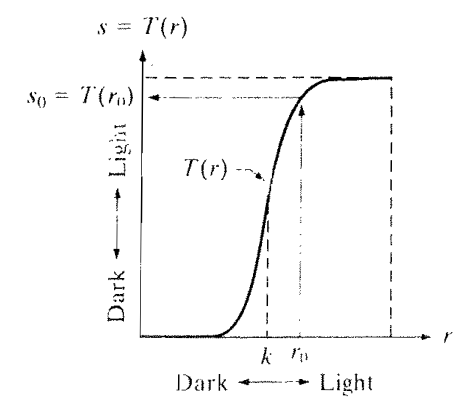
\includegraphics[width=1\textwidth]{images/03/01.png}
    \end{tabular}
  \caption{\label{fig:contrast} Aumento de contraste}
\end{subfigure}
\begin{subfigure}{.5\textwidth}
  \centering
    \begin{tabular}{c}
      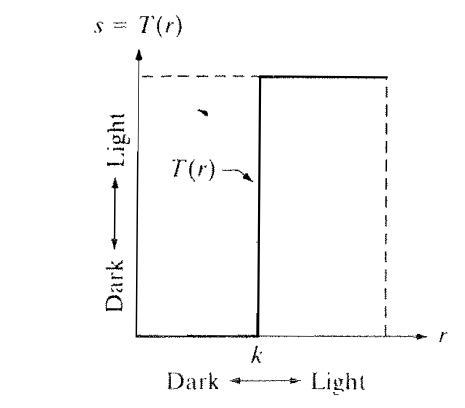
\includegraphics[width=1\textwidth]{images/03/02.png}
    \end{tabular}
  \caption{\label{fig:thresh} \textit{Threshold}}
\end{subfigure}
\caption{\label{fig:gray} \textit{Gray-level transformations}}
\end{figure}


%%%%%%%%%%%%%%%%%%%%%%%%%%%%%%%%%%%%%%%%%%%%%%%%%%%%%%%%%%%%
\section{\emph{Gray-level transformations} simples}

\begin{easylist}

  & Negação: ver Figura~\ref{fig:gray2}.
  \[ s = L-1-r \]
  & Transformações logarítmicas: ver Figura~\ref{fig:gray2}.
  \[ s = c \log(1+r) \]
  & Transformações por potenciação: ver Figura~\ref{fig:power}.
  \[ s = cr^\gamma \]
  & \textit{Piecewise linear transformations}: ver Figura~\ref{fig:piece}.

\end{easylist}

\begin{figure}[!h]
  \begin{center}
    \begin{tabular}{c}
      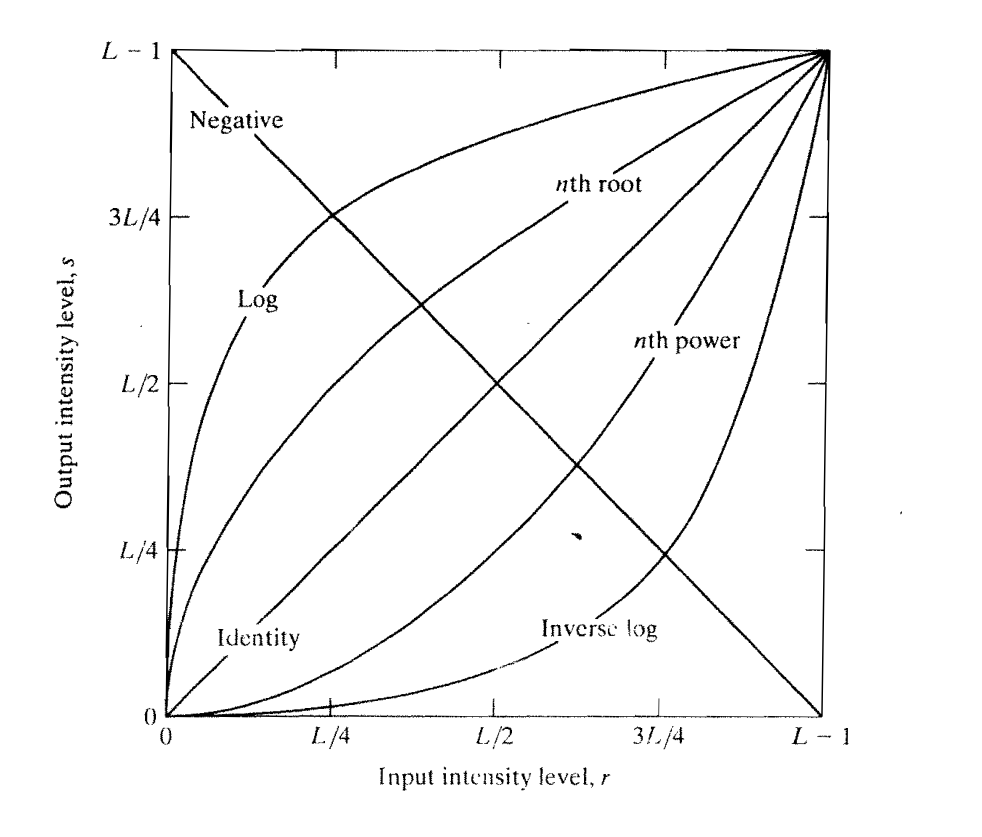
\includegraphics[width=0.8\textwidth]{images/03/03.png}
    \end{tabular}
  \end{center}
  \caption{\label{fig:gray2} Exemplos de \textit{gray-level transformations} simples.}
\end{figure}

\begin{figure}[!h]
  \begin{center}
    \begin{tabular}{c}
      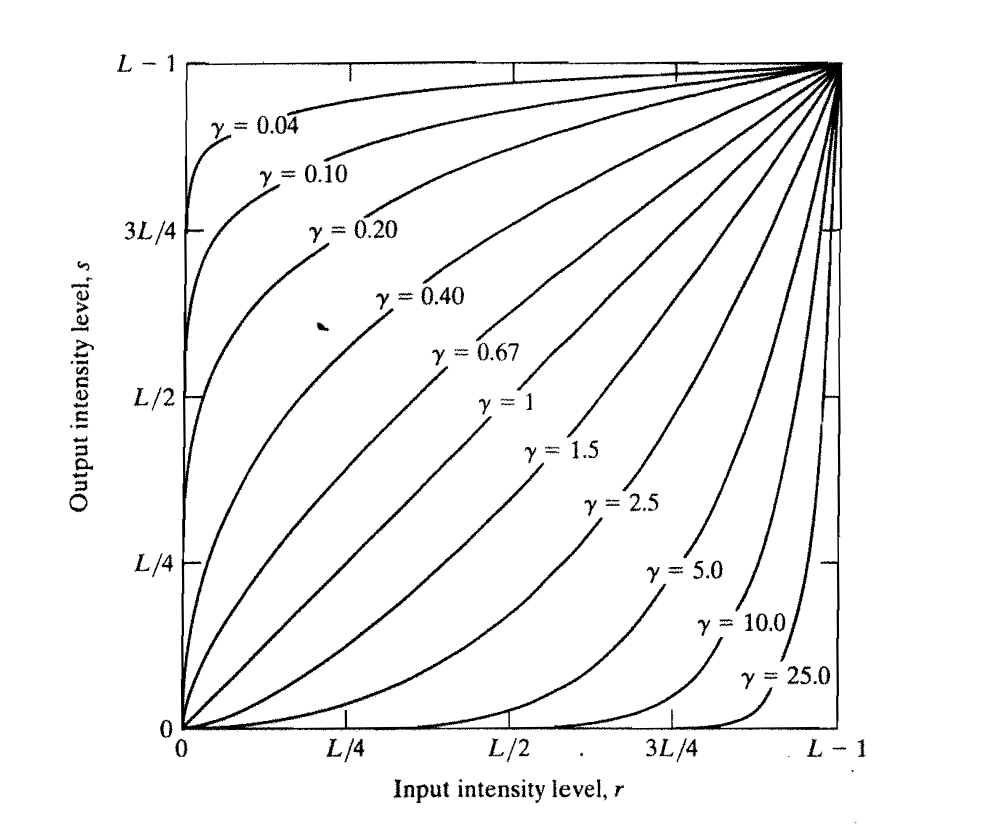
\includegraphics[width=0.8\textwidth]{images/03/04.png}
    \end{tabular}
  \end{center}
  \caption{\label{fig:power} Transformações por potenciação com diferentes expoentes}
\end{figure}

\clearpage

\begin{figure}[!h]
  \begin{center}
    \begin{tabular}{c}
      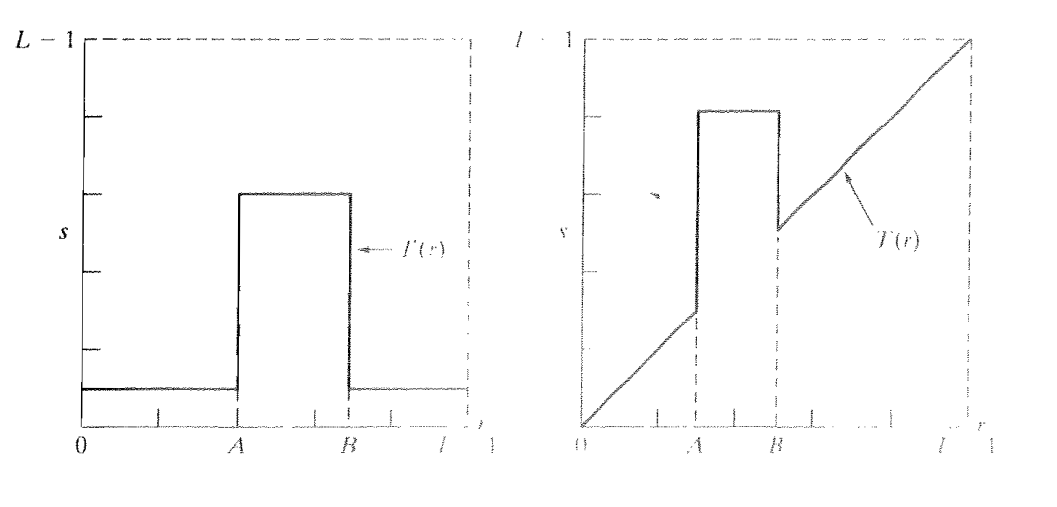
\includegraphics[width=0.9\textwidth]{images/03/05.png}
    \end{tabular}
  \end{center}
  \caption{\label{fig:piece} \textit{Piecewise linear transformations}}
\end{figure}


%%%%%%%%%%%%%%%%%%%%%%%%%%%%%%%%%%%%%%%%%%%%%%%%%%%%%%%%%%%%
\section{Processamento de histograma}

\begin{easylist}

  & Histograma: de uma imagem digital com tons de cinza no intervalo $[0, L-1]$ é uma função discreta $h(r_k) = n_k$, onde $k$ é o $k$-ésimo tom de cinza, $r_k = k / (L-1)$ e $n_k$ é o número de pixels na imagem com tom de cinza igual a $k$.

  & Histograma normalizado: é dado por $p(r_k) = n_k / n$, onde $n$ é o total de pixels da imagem.

  & Equalização de histograma: é uma transformação que distribui uniformemente as escalas de cinza pelo intervalo dinâmico.

  \[ s = T(r), 0 \leq r \leq 1 \].

  && T(r) tem valor único e é monotonicamente crescente no intervalo $0 \leq r \leq 1$.

  && $0 \leq T(r) \leq 1$ para $0 \leq r \leq 1$.

  A probabilidade de ocorrência de um tom de cinza na imagem é

  \[ p(r_k) = n_k / n, k \in [0, L-1] \]

  \[ T(r_k) = \sum_{j=0}^k p(r_j) = \sum_{j=0}^k \frac {n_j}{n} \]
  
\end{easylist}


%%%%%%%%%%%%%%%%%%%%%%%%%%%%%%%%%%%%%%%%%%%%%%%%%%%%%%%%%%%%
\section{Operações aritméticas e lógicas}

\begin{easylist}

  & Interseção ou \textit{AND} lógico ou mínimo entre duas imagens: útil para aplicar máscaras.

  & Subtração: útil em imagens médicas com contraste radioativo.

  & Média: útil para diminuir o ruído quando é possível tirar várias fotos de um mesmo ponto de vista. Aplicada em astronomia.
  
\end{easylist}


%%%%%%%%%%%%%%%%%%%%%%%%%%%%%%%%%%%%%%%%%%%%%%%%%%%%%%%%%%%%
\section{Filtragem espacial}

\begin{easylist}

  & Filtragem espacial linear: é dada pela soma de pixels multiplicados por pesos
  && Correlação:

  \[ g(x, y) = \sum_{s = -a}^a\sum_{t = -b}^b w(s, t) f(x+s, y+t) \]

  onde $g$ é a imagem de saída, $(2a+1)(2b+1)$ é o tamanho do filtro, máscara, \textit{kernel} ou janela, e $f$ é a imagem de entrada.
  
  && Convolução:

  \[ g(x, y) = \sum_{s = -a}^a\sum_{t = -b}^b w(s, t) f(x-s, y-t) \]

  & Filtragem espacial não-linear: mediana, variância, filtros morfológicos dentre outros.
  
\end{easylist}

  

